\subsection{Experiments}

\label{sec:exps}
\subsection{Datasets}

In this work two popular face verification datasets were used. We use Labeled Faces in the Wild (LFW) to evaluate the \textit{baseline architecture}, which closely follows \cite{TuzelTH16} but is trained using \emph{Perceptual loss} (see section \ref{sec:loss} for details). Our multi-frame architecture described in section~\ref{sec:video} is evaluated using YouTube Faces dataset. The ablation study on the same dataset include evaluation of different architecture variants described in section~\ref{sec:arch}.

Labeled Faces in the Wild (LFW) \cite{KaramZ15} contains 13,233 images with 5,749 identities. The standard evaluation procedure for LFW includes similarity estimation for the given set of image pairs. All pairs are split into ten subsets non-overlapping in terms of identities. We use standard test subset $1$ to evaluate our super-resolution methods. Identities that are not included into test subset $1$ are thus used for training. To evaluate the recognition quality, we use the Equal Error Rate (EER) (i.e.\ the error rate at the ROC operating point where the false positive and false negative rates are equal). To get EER values, we first  compute descriptors for the face images using pre-trained face recognition model \cite{ParkhiVZ15}.
%TODO : how many persons in train/test

%EER does not depend on the similarity threshold that separates similarity values for 'positive' and 'negative' pairs of images. 

To evaluate our video-based super-resolution method, we use the YouTube Faces (YTF) dataset \cite{WolfHM11}. It contains 3,425 videos of 1,595
people collected from YouTube, with an average of 2 videos per identity. Similarly to LFW, EER is used to evaluate recognition quality for the YTF dataset. The only difference is that the similarity value is estimated for each pair of videos. To do this, we calculate the mean similarity for all pairs of frames of the two tracks. As this is time-consuming operation, we take only first $100$ frames in each video (the first $20$ frames were used for comparison with \cite{ZhuLLT16}). %The number of the frames used for the evaluation is less because we only take those frames that at least have $12$ neighboring subsequent frames before and after them. This is done to compare results for different variants of the video-based super-resolution method.

We also use PSNR (for luminance channel) and Euclidean distance metrics for comparing different variants of model described in \ref{sec:video}. We use $623$ images from the YTF dataset to compare PSNR and Euclidean distance between features of ground truth and reconstructed images extracted using VGG face model layers \emph{pool3}, \emph{pool4} and \emph{fc7}.

All experiments were performed by considering the downsampled versions of images from the described datasets as inputs. Unless specified otherwise, we give results are for input of size 16$\times$16 and output of size 128$\times$128, so the upsampling is upto $\times$8. It is a very challenging setting, which still allows to see meaningful variations between methods (much higher magnification factors result in all methods performing equally bad, and much lower magnification factors result in all methods performing equally well).

\subsection{Architectures}

\label{sec:arch}
The following architectures were used in our experiments:
\begin{enumerate}
    \item The single-image architecture from \cite{TuzelTH16} denoted \texttt{f$1$} ( \emph{8$\times$GN} and  \emph{8 layer LN} were used for \emph{Local} and \emph{Global} modules of the architecture).
    \item The multi-frame architecture similar to described in Section~\ref{sec:video} but without \emph{Face Warping} subnetwork. This architecture stacks features for all frames  without alignment and then processes the stack by the \emph{Reconstruction} subnetwork. We experiment with two variants of this architecture \texttt{f$5$} and \texttt{f$25$} that accept sequences of length $5$ and $25$ accordingly.
    \item The full multi-frame architecture described in Section~\ref{sec:video} is also implemented in two variants \texttt{f$5$warp} and \texttt{f$25$warp} that accept sequences of length $5$ and $25$ accordingly.
\end{enumerate} 
The single-image architecture \cite{TuzelTH16} is evaluated for the LFW dataset and several modes of using \emph{Perceptual} loss are compared in the section \ref{sec:perceptual}.
The proposed multi-frame architecture (section \ref{sec:video}) is evaluated on the YTF dataset.
Further details of the architectures are discussed below.



\subsection{Training the model}

The \emph{feature extractor} sub-network is implemented similar to \emph{8$\times$GN} in \emph{Global} module in \cite{TuzelTH16}. It includes two parallel streams. The first stream performs upsampling using one deconvolution layer, while the second stream consists of four fully connected layers. The first three fully connected layers have $256$ neurons, while the last one has the size $128\times128$.

The \emph{face warping} sub-network accepts pairs of images. Initially, the two images are processed separately using  two sub-networks consisting of three convolution layers with $20$ filters of sizes $3\times3$, $3\times3$ and $1\times1$ accordingly. The outputs of these two streams are concatenated and passed to the next five convolution layers with $100$ filters of size $3\times3$ each.
Then three fully connected layers with $256$ neurons are applied. The final fully connected layer then outputs shifts for coordinate pairs of $64$ control points. The warping is performed using thin plate spline with $64$ control points located in the nodes of the regular grid \cite{JaderbergSZK15}.

The \emph{reconstruction} sub-network is implemented similarly to \emph{Local} module in \cite{TuzelTH16}. It consists of eight convolution layers:
\vspace{5mm}
\begin{tabular}{c |c c c c c c c c }
\hline
  \#conv & 1& 2& 3 & 4 & 5&6  & 7 &8 \\
  \#filters & $16$ & $32$&$64$&$64$&$64$&$32$&$16$&$3$  \\
  filter size &$5$& $7$& $7$& $7$& $7$& $7$& $5$& $5$ \\
\hline
\end{tabular}

ReLU (rectified linear unit) activation functions are used for all the layers except the last convolution layer in the \emph{Reconstruction} sub-network. The latter uses the sigmoid activation.

The architecture is trained using \ref{eq:loss} and the ADAM optimizer~\cite{KingmaB14} for ~1,500 epochs with learning rate fixed to $1e-4$. Batch size is set to $10$. Pre-trained VGG-16 face model from \cite{ParkhiVZ15} is used for calculating deep features within loss \ref{eq:loss}. We normalize all the features before calculating the loss value \ref{eq:loss}, otherwise the training process get stuck in bad local minima.

The \emph{face warping} sub-network is pre-trained in unsupervised manner using pairs of images. The L1 loss for the warped and reference images is used for training.

For the LFW dataset, we used $\lambda_{pool3}$, $\lambda_{pool4}$ and $\lambda_{fc7}$ set to $10^3$ for the loss \ref{eq:loss}. For the YTF dataset, the value of $10^5$ was used because the quality of ground-truth images in YTF is much worse than for LFW and therefore pixel-level loss is less useful for the training on YTF. Increasing values of $\lambda_{pool3}$ and $\lambda_{pool4}$ also affects the color of resulting images, as deep features are more color-independent (c.f.~\ref{fig:ytube}, row $5$, where the green background became grey in the reconstruction). 





\subsection{Perceptual Loss effects}
\label{sec:perceptual}


First, we experimented with training the baseline single-image super-resolution ConvNet (the architecture from \cite{TuzelTH16}) using the Perceptual loss in addition to the pixel-level loss. Here we show some of the results that demonstrate the effect of using deep features extracted from different layers of the pre-trained VGG-face model and choose the most beneficial variant.

As mentioned above, we evaluate the models using the split 1 of the LFW dataset. All images were resized to $128\times128$ pixels, blurred (Gaussian kenel, $\sigma=2.4$) and downsampled to $16\times16$ pixels for training and testing.

%It turned out that using fully-connected layers of the pre-trained VGG-face model leads to the decreasing image quality. See Figure \ref{fig:fc7} for results of learning with perceptual loss using \emph{fc7} layer of the VGG-face model additionally to the pixel-level L2 loss. 

The most visually plausible results were achieved by using the \emph{pool3} and \emph{pool4} layers for learning along pith pixel-level data. The results on LFW hold-out set were compared with bicubic interpolation as well as with the variant learned with pixel-level loss only. The comparison in Figure \ref{fig:layers} shows clear improvement of the system that uses pixel-level loss over the baselines. 

We also observed that using perceptual loss improved the recognition score. Recognition scores ($100\%$-EER) for these cases are compared in  \ref{tab:lfw_score}. At the same time, as expected, best results in terms of PSNR (peak signal-to-noise ratio) were achieved with pixel-level loss. %TODO : insert values

%Additionally, we have compared the results for down-sampling factor $4$ (input images were of size $32\times32$), but there was no difference in either visual quality or recognition score between the results \emph{pixel} and \emph{pixel} $+$ \emph{pool3} $+$ \emph{pool4} modes.




\begin{table*}
\centering
\begin{tabular}{ c | c c c c c }
  & gt & bicubic & \emph{pixel}  & \emph{pixel} + \emph{pool3} + \emph{pool4} & \emph{pixel} + \emph{fc7}  \\
\hline
train & -      & -    & 85.56 & 86.19 & 90.74\\
test  & 95.33 & 73.01 & 83.02 & \bf{85.02} & 84.33\\


\end{tabular}
\caption{100\% - EER (Equal error rate) values for the standard split $1$ of the FLW dataset. The scores for bicubic upsamling and ground truth images are also included. \emph{pixel} - the results achieved using pixel-level loss only. Best results were achieved using pixel-level loss along with \emph{Perceptual} loss for layers \emph{pool3} and \emph{pool4} of the pre-trained VGG-face model.}
\label{tab:lfw_score}
\end{table*}



% \begin{figure*}
% \begin{center}

% \includegraphics[width=\textwidth]{\srroot/images/lfw/fc7.png}

% \caption{The results achieved by training the super-resolution network using additional perceptual loss term that compares reconstruction and ground truth images representations extracted from the \emph{fc7} layer of the pre-trained VGG-face model. No image quality improvement is observed, on the contrary, images become less realistic with the increase of perceptual loss weight. }

% \label{fig:fc7}

% \end{center}

% \end{figure*}



\begin{figure}[t]



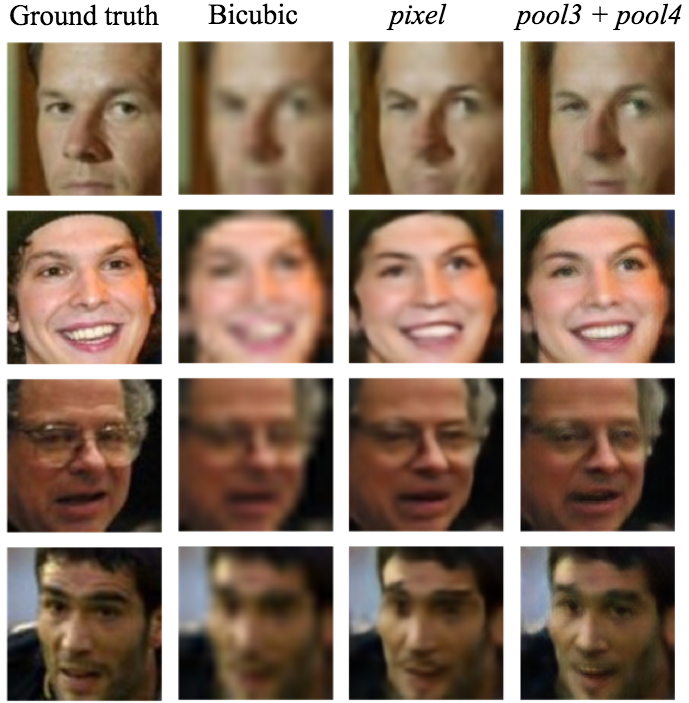
\includegraphics[width=\columnwidth]{\srroot/images/lfw/layers_short.png}

\caption{The results achieved using additional \emph{Perceptual} loss terms for layers \emph{pool3} and \emph{pool4} compared with result for pixel-level loss and bicubic interpolation. We can see the clear improvement when using layers \emph{pool3} and \emph{pool4} along with pixel-level data.}

\label{fig:layers}



\vspace{10pt}
\end{figure}

\subsection{Experiments with video-data}

We have performed experiments on video-based face super-resolution using different variants of face super-resolution network described in \ref{sec:video}. All images were fist resized to $128\times128$ pixels, blurred with the Gaussian kernel ($\sigma = 2.4 $), and downsampled to the size $16\times16$. 
Here we use previously chosen perceptual loss training mode \emph{pixel} + \emph{pool3} + \emph{pool4} that uses pixel-level differences along with differences of features at \emph{pool3} and \emph{pool4} layers to compute the final loss value. The weight equal to $10^5$ was used for both Perceptual loss components  \emph{pool3} and \emph{pool4}.


In \ref{tab:ytube_score} $100\%-$EER(Equal Error Rate) value for single-image super-resolution is compared to video-based results using different number of adjacent frames with and without frame alignment (warping). Values for ground truth images (without distortions) and bicubic upsampling are also included. Note, that ground truth performance is less than reported in \cite{ParkhiVZ15} for several reasons: we use only one scale $256\times256$ and only one crop (central) to calculate face image descriptor. Moreover, all ground truth images were resized to $128\times128$ pixels to make fair comparison with our super-resolution method that outputs images of this size. 

The best-performing method was \texttt{f$25$warp} that uses 25 frames (one central and $24$ neighboring ones) and frame warping. Using several frames is generally better than using only one frame (c.f.~super-resolution results comparison in \ref{fig:ytube}). In \ref{tab:ytube_score} we can also see that the architecture \texttt{f$25$warp} gives reconstruction that are the closest to ground-truth when comparing images using L2 distance between their VGG deep features. The best PSNR value was achieved using \texttt{f$5$warp}. In general, we can see uniform improvement in all used metrics (with the exception of PSNR) for architectures that use longer sequences in comparison to architectures that use less frames. Analogously, there is improvement for architectures that include \emph{Face Warping} module (\texttt{f$25$warp} and \texttt{f$5$warp}) in comparison to architectures without \emph{Face Warping} module (\texttt{f$25$} and \texttt{f$5$}).



\begin{table*}
\centering
\begin{tabular}{c | c c c c c c c c}
 metric & gt & bicubic & \texttt{f$1$} & \texttt{f$5$} &  \texttt{f$25$} & \texttt{f$5$warp} &  \texttt{f$25$warp}  \\
\hline
$100$\%-EER & 85.60 & 78.80 & 82.40 & 83.20 & 83.60 & 84.39 & \bf{85.20}\\
PSNR      && & 27.64 & 28.22 & 28.28 &  \bf{29.17} & 29.12 \\
L2, \emph{pool3} &&& 0.6512 & 0.6199 & 0.6295 & 0.5568 &  \bf{0.5542} \\
L2, \emph{pool4} &&& 0.7110 & 0.6814 & 0.6918 & 0.6126 &  \bf{0.6074} \\
L2, \emph{fc7} &&& 0.4828 & 0.4478 & 0.4583 & 0.3811 &  \bf{0.3695} \\




\end{tabular}
\caption{Different metrics for several architectures evaluated in this work (see section \ref{sec:arch}). First row (face verification metric): 100\%-EER(Equal error rate), second row: PSNR - peak signal to noise ratio. Rows $3$-$5$ show mean Euclidean distances between deep features of ground truth and reconstructed images extracted using VGG-face layers \emph{pool3}, \emph{pool4}, \emph{fc7} (after normalization). Such metrics are strongly correlated with recognition. The best performing architecture is \texttt{f$25$warp} that accepts sequences of length $25$ and includes \emph{Face Warping} sub-network. See section \ref{sec:video} for details.}
\label{tab:ytube_score}
\end{table*}

\subsection{User study for multi-frame face super-resolution}
\label{sec:ustudy}


We also carried out a user study in order to compare human perception of images produced by architectures \texttt{f$1$}, \texttt{f$25$} and \texttt{f$25$warp}. 
We thus compared the following three pairs of architectures: \texttt{f$25$} vs \texttt{f$25$warp}, \texttt{f$1$} vs \texttt{f$25$warp}, \texttt{f$1$} vs \texttt{f$25$}. The comparison interface presented five result pairs (for each of the three pairs of methods) from the YTF dataset to each user. Within the pair, the order was randomized. Between the pair, we showed a full-resolution frame from the same sequence (different from the central frame). The users were asked to pick one of the two reconstruction that (a) resemble the reference image more and (b) has better overall quality. The users were asked to prioritize resemblance over visual quality. Finally, if the two images seemed to the user absolutely on par both in terms of resemblance and quality, the user were allowed to click on the middle (reference) frame to indicate this. We however asked the users to abstain from this as much as possible. Overall $42$ users took part in the study.

%Second criterion (less important) was the overall image quality. In addition to two images that can be chosen, users could also answer "none", meaning that it is hard to decide which of the images is better.

The results of the user study (\ref{fig:ustudy}) showed that it is easy to tell the difference between the results of  \texttt{f$25$} vs \texttt{f$25$warp}  and \texttt{f$1$} vs \texttt{f$25$warp}. It appeared to be challenging to differ \texttt{f$1$} vs \texttt{f$25$} methods. These observations indicate that \emph{Face Warping} module is essential for obtaining better results. Using more frames without warping thus did not bring advantage over single-frame super-resolution.

\begin{figure}[t]

\begin{center}
    

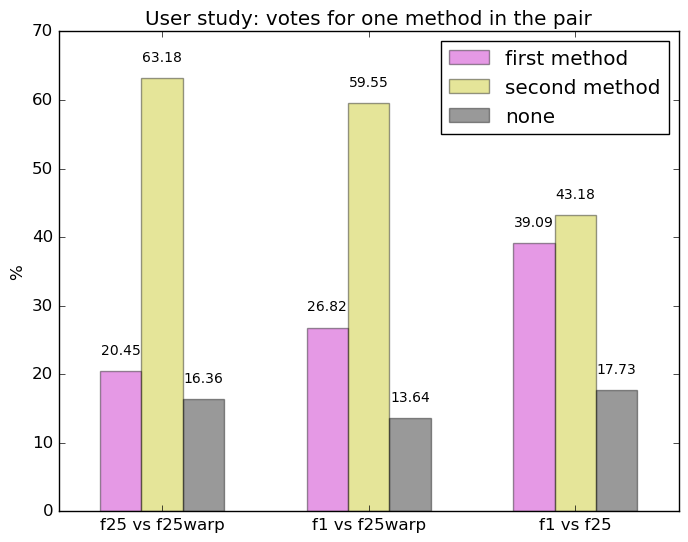
\includegraphics[width=\columnwidth]{\srroot/images/ytube/ustudy.png}
\end{center}
\caption{Results of user study for the three pairs of architectures evaluated in this works. See details in section \ref{sec:ustudy}}

\label{fig:ustudy}



\vspace{10pt}
\end{figure}




\subsection{Comparison to state of the art}

Here we compare our method with one of the latest single-image super-resolution methods \cite{ZhuLLT16}. As we use different format of input images than in \cite{ZhuLLT16} (for example, we use tighter crops for faces), we evaluate \cite{ZhuLLT16} on the YTF dataset using less magnification factor than we use in this work. For our methods we use inputs of size $16\time16$, while using $32\times32$ for \cite{ZhuLLT16}. We use the code published for \cite{ZhuLLT16} for the evaluation and therefore ensure that all the inputs are preprocessed as appropriate for \cite{ZhuLLT16} (including face detector for cropping the ground truth images from initial frames). As in \cite{ZhuLLT16}, the downsampled images were created without applying gaussian blur beforehands, we perform the comparison on such images after retraining our architecture for such regime. 

We observed that our method performs better than \cite{ZhuLLT16} in terms of $100$\%-EER metric: 85.14 (ours) vs 82.32 (\cite{ZhuLLT16}). Also, we can see that $100$\%-EER value for \cite{ZhuLLT16} is very close to the $100$\%-EER value for \texttt{f$1$} architecture that we use as a single-image baseline in this work (see Table \ref{tab:ytube_score}).
%TODO maybe insert L2 varues, but we need to change the code in \cite{ZhuLLT16} so that it wouldnt rotate the images.




\begin{figure*}
\begin{center}

\includegraphics[width=0.8\textwidth]{\srroot/images/ytube/ytube.png}

\caption{Results of different super-resolution CNNs for some of the images in the YTF dataset. Ground truth images and bicubic upsampling results are in the first two columns. See sections \ref{sec:arch} and \ref{sec:video} for details.}

\label{fig:ytube}

\end{center}

\end{figure*}